\section{Resultados y Análisis}

Este capítulo consolida los resultados funcionales, técnicos y de validación con usuarios obtenidos durante el cierre del proyecto. La evidencia se organiza en cuatro frentes: estado funcional de la build WebGL, rendimiento técnico por dispositivo, evaluación de usabilidad/carga de trabajo con 12 participantes anonimizados y resultados del pipeline de activos 3D. La lectura cuantitativa se mantiene descriptiva y formativa, coherente con el tamaño y tipo de muestra, pero se apoya en datos fechados y trazables de la build publicada.

\subsection{Estado de cierre funcional}

La build final publicada integra el flujo principal previsto para el MVP académico: ingreso desde el Hero, onboarding, exploración orbital, selección de piezas, \textit{bottom sheet} de información, hotspots, aislamiento, modos \textit{Inspect}/\textit{Analyze}/\textit{Studio}, corte transversal, vista explosionada, filtros por categoría y visualización térmica heurística. La revisión funcional posterior a las correcciones P1/P2 confirmó que el flujo visible corresponde con lo descrito en los manuales y con la arquitectura documentada en el capítulo de desarrollo.

La revisión funcional se complementa con mediciones técnicas y con instrumentos de usuario aplicados posteriormente. Por ello, la Tabla \ref{tab:estado_cierre_funcional} resume el cierre operativo de la app, mientras que las subsecciones siguientes reportan los datos de rendimiento, SUS, NASA-TLX Raw y \textit{Think-Aloud}.

\begin{table}[p]
    \caption{Estado de cierre funcional por frente de validación}
    \label{tab:estado_cierre_funcional}
    \centering
    \footnotesize
    \setlength{\tabcolsep}{3pt}
    \renewcommand{\arraystretch}{0.8}
    \begin{tabular}{>{\RaggedRight\arraybackslash}p{3.15cm}>{\RaggedRight\arraybackslash}p{3.05cm}>{\RaggedRight\arraybackslash}p{5.05cm}>{\RaggedRight\arraybackslash}p{2.45cm}}
        \hline
        \textbf{Frente} & \textbf{Estado} & \textbf{Evidencia de cierre} & \textbf{Dato de validación} \\ \hline
        Flujo principal WebGL & QA funcional correcto & La app permite explorar, seleccionar, aislar, analizar y volver al menú sin romper el flujo visible & Métricas por escenario \\
        Interacción móvil & QA P1/P2 correcto & Gestos, \textit{bottom sheet}, doble toque, zoom, órbita e iconos fueron ajustados tras observación directa & Tabla por dispositivo \\
        Rendimiento percibido & Correcto en revisión formativa & La app se observó fluida en escritorio y en la mayoría de móviles de gama media-baja probados, incluyendo Redmi Note 10S & FPS, memoria y carga \\
        Usabilidad formativa & Correcta para cierre iterativo & La prueba breve permitió convertir gestos espontáneos en ajustes concretos de interfaz & SUS, NASA-TLX y \textit{Think-Aloud} \\
        Manuales e informe & Coherencia revisada & La documentación distingue funciones visibles, capacidades ocultas y resultados de validación & Datos de campo registrados \\ \hline
    \end{tabular}
    \par\vspace{0.5\baselineskip}
    \apanote{Esta tabla resume el cierre funcional y no reemplaza las tablas cuantitativas posteriores. Elaboración propia.}
\end{table}

\subsection{Aporte frente a necesidades de la industria de hardware complejo}

La revisión conceptual de cierre permitió reinterpretar los resultados funcionales del prototipo frente a necesidades recurrentes de la industria de hardware complejo. El producto no debe evaluarse únicamente como una escena 3D, sino como una primera capa de comprensión espacial, comunicación técnica y preparación semántica de componentes. En ese sentido, la build final cubre parte de las necesidades de inspección, soporte inicial, entrenamiento y demostración del producto, aunque todavía no cubre telemetría, diagnóstico, mantenimiento guiado ni interoperabilidad industrial completa (véanse la Tabla \ref{tab:necesidades_industriales_respuesta_prototipo} y la Figura \ref{fig:necesidades_respuesta_evolucion}).

\begin{table}[H]
    \caption{Relación entre necesidades industriales y respuesta del prototipo}
    \label{tab:necesidades_industriales_respuesta_prototipo}
    \centering
    \scriptsize
    \begin{tabular}{p{3.3cm}p{5.1cm}p{4.0cm}p{2.1cm}}
        \hline
        \textbf{Necesidad industrial} & \textbf{Respuesta actual del proyecto} & \textbf{Límite vigente} & \textbf{Madurez} \\ \hline
        Comprensión espacial de hardware complejo & Navegación 3D, selección, aislamiento, vista explosionada, corte y modos de inspección & Se complementa con documentación técnica, validación por tareas e instrumentos de usuario & Visual product twin \\
        Transferencia de conocimiento técnico & Onboarding, hotspots, fichas por pieza, categorías y flujo mobile-first & Falta medir formalmente aprendizaje longitudinal o retención posterior & Visual product twin \\
        Conversión CAD a activo web & Pipeline CAD/Blender/Unity, saneamiento runtime, presupuesto geométrico y profiler interno & La reducción geométrica se reporta por rutas de importación y optimización & Digital model semántico \\
        Datos de producto fragmentados & Taxonomía 28/30/257, grupos de escena y fichas como base de identificadores & No existe aún \textit{twin manifest} formal ni conectores externos & Preparación semántica \\
        Soporte y mantenimiento & Selección contextual y lectura por componentes pueden servir como base de procedimientos & No hay síntomas, repuestos, historial, órdenes de trabajo ni reglas de diagnóstico & Trabajo futuro \\
        Estado operacional y telemetría & Visualización térmica heurística introduce la idea de estado por componente & No hay telemetría real, calibración física ni sincronización con activo & Pre-shadow conceptual \\ \hline
    \end{tabular}
    \par\vspace{0.5\baselineskip}
    \apanote{La tabla distingue respuesta funcional actual, límite técnico y nivel de madurez. No clasifica la build como \textit{digital twin} operacional. Elaboración propia a partir de la investigación conceptual y la build final.}
\end{table}

\begin{figure}[H]
    \caption{Necesidades industriales, respuesta actual y evolución futura defendible.}
    \label{fig:necesidades_respuesta_evolucion}
    \centering
    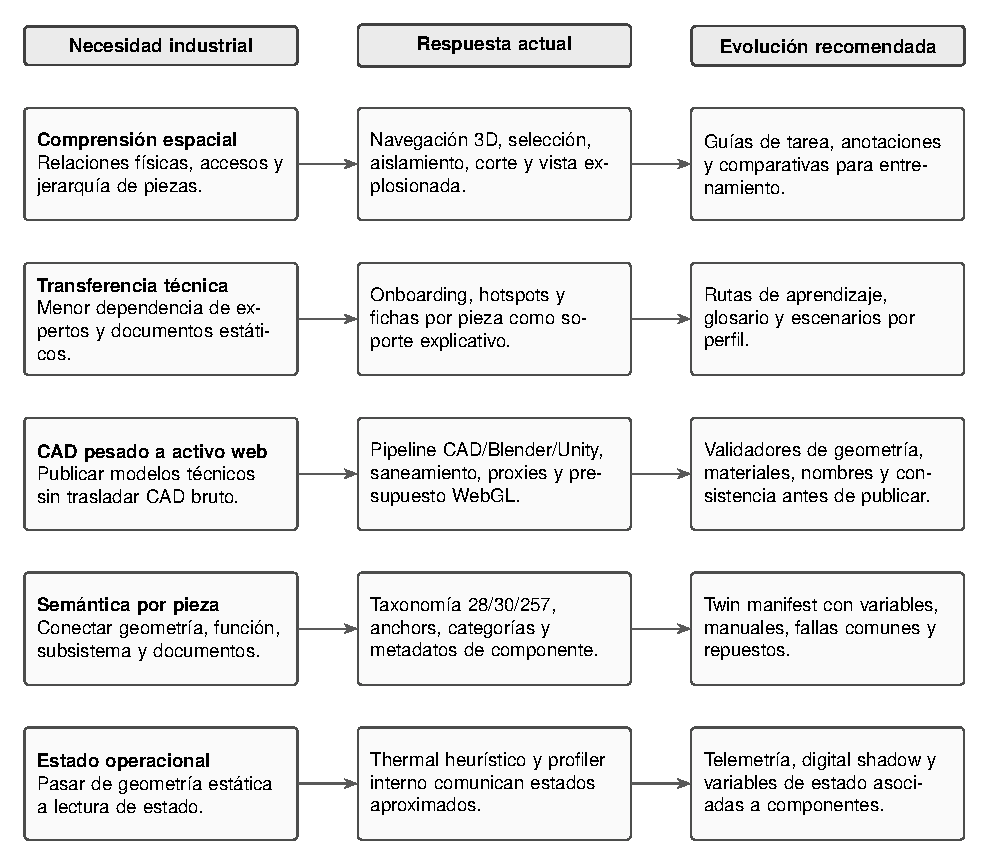
\includegraphics[width=\textwidth,height=0.82\textheight,keepaspectratio]{figures/apa_redesign/fig_apa_necesidades_respuesta_evolucion.pdf}
    \par\vspace{0.5\baselineskip}
    \apanote{La lectura va de izquierda a derecha: necesidad industrial, capacidad ya entregada y evolución recomendada. La figura no clasifica la build actual como \textit{digital twin} operacional. Elaboración propia.}
\end{figure}

Esta lectura fortalece la justificación del proyecto: el dron Holybro X500~V2 opera como caso representativo de un sistema electromecánico multicomponente, pero el problema de fondo es transferible a maquinaria, robótica, equipos técnicos, plataformas motorizadas e instrumentos con integración mecánica, eléctrica, electrónica, sensorial y de control. La contribución actual consiste en demostrar una capa visual-semántica usable y desplegable en web; la contribución futura dependerá de conectar esa capa con datos operativos y procedimientos de servicio.

\subsection{Resultados formativos de rendimiento}

El cierre técnico incorporó un profiler interno capaz de registrar sesiones por escenario y exportarlas en JSON o CSV. Cada sesión permite asociar la experiencia de uso con FPS promedio, \textit{frame time}, peor \textit{frame time}, memoria, resolución, plataforma, dispositivo, navegador, modo visual, factor de explosión, corte transversal, cantidad de renderers, mallas y triángulos estimados. Esta instrumentación resuelve el problema metodológico de depender únicamente de impresiones subjetivas o de herramientas externas.

Durante la revisión directa de la build se observó que la optimización es adecuada para el alcance del MVP: la aplicación se mantuvo fluida en escritorio y funcional en móviles reales de gama media, con Redmi Note 10S como referencia representativa compartida durante el cierre. Esta afirmación se limita al comportamiento observado y se complementa con el resumen por dispositivo de la Tabla \ref{tab:rendimiento_webgl_resumen_dispositivos}, con los KPIs complementarios de la Tabla \ref{tab:kpis_complementarios_build_memoria} y con el detalle de sesiones de la Tabla \ref{tab:rendimiento_webgl_detalle_sesiones}. Estas tablas proceden de exportaciones fechadas del profiler interno de la app y de artefactos publicados de la build, por lo que separan medición técnica, lectura interpretativa y exclusiones justificadas. En los casos en que Unity WebGL normaliza el sistema operativo en la exportación del profiler, la identificación del entorno se contrasta con el registro manual de dispositivo, sistema operativo, navegador y resolución.

% Tablas generadas a partir de los archivos en:
% Telemetria/Mediciones_WebGL
%
% Criterio de procesamiento:
% - FPS promedio y frame time promedio se calcularon como promedios ponderados
%   por duración a partir de los campos exportados por el profiler interno.
% - Se excluyeron de los agregados los segmentos identificados como arranque
%   corto, captura accidental o suspensión atípica del navegador.
% - Se excluyó la captura Chrome 91 con peor frame de 87699 ms por ser una
%   sesión atípica compatible con pausa, background o suspensión del navegador.
% - Unity WebGL reportó algunos navegadores móviles como deviceType=Desktop; la
%   clasificación de dispositivo se hizo por sistema operativo, navegador, GPU y
%   resolución.

\begin{table}[H]
    \caption{Resumen de rendimiento WebGL por dispositivo y escenario operativo}
    \label{tab:rendimiento_webgl_resumen_dispositivos}
    \centering
    \scriptsize
    \singlespacing
    \renewcommand{\arraystretch}{1.08}
    \setlength{\tabcolsep}{2pt}
    \begin{tabular}{p{2.5cm}p{2.1cm}p{2.65cm}p{0.9cm}p{1.05cm}p{1.25cm}p{1.1cm}p{2.15cm}}
        \hline
        \textbf{Dispositivo} & \textbf{SO / navegador} & \textbf{Escenarios válidos} & \textbf{Dur. (s)} & \textbf{FPS prom.} & \textbf{Frame prom.} & \textbf{Pico mem.} & \textbf{Lectura} \\ \hline
        PC escritorio (Intel Core i7-5820K, GTX 980 Ti, 48 GB RAM), 1910\(\times\)903 & Windows 11 / Chrome 141 & Base, selección/aislamiento, explode, cut, thermal/studio & 253.4 & 59.8 & 16.7 ms & 413 MB & Fluidez estable en todos los escenarios operativos. \\
        Móvil Android (Adreno 610), 720x1300 & Android 10 / Chrome 148 & Base, selección/aislamiento, explode, cut, thermal/studio & 389.5 & 24.5 & 52.1 ms & 311 MB & Rendimiento usable, con picos perceptibles y thermal/studio como escenario más exigente. \\
        Móvil Android (Adreno 610), 720x1410 & Android 12 / Chrome 114 & Base, selección/aislamiento, explode, cut, thermal/studio & 115.4 & 17.6 & 61.4 ms & 263 MB & Límite inferior móvil: navegable, pero por debajo de la meta de 30 FPS. \\
        Móvil Android (Adreno 650), 1280x1914 & Android 12 / Chrome 114 & Base, selección/aislamiento, explode, cut, thermal/studio & 149.8 & 30.0 & 36.2 ms & 254 MB & Cerca de la meta de 30 FPS, con picos aislados durante cut. \\
        Redmi Note 10S (Mali-G76), 924x1862 & MIUI Global 14.0.11 / Chrome 148 & Base, selección/aislamiento, thermal/studio, explode, cut & 156.7 & 26.5 & 40.3 ms & 226 MB & Experiencia móvil funcional en el flujo principal. \\
        iPhone 17 Pro (A19 Pro), 1206x2622 & iOS / Safari & Base, selección/aislamiento, explode, cut, thermal/studio & 180.0 & 58.7 & 17.0 ms & 356 MB & Fluidez cercana al objetivo de 60 FPS en recorrido completo. \\
        Móvil Android (Adreno 650), 1280x1808 & Android 12 / Chrome 91 & Base & -- & -- & -- & 119 MB & Captura descartada del agregado por comportamiento atípico de pausa o suspensión. \\ \hline
    \end{tabular}
    \par\vspace{0.5\baselineskip}
    \apanote{Los promedios se calcularon sobre sesiones operativas exportadas por el profiler interno de la app. Se excluyeron segmentos de arranque corto, capturas accidentales y una captura atípica de Chrome 91 con peor frame de 87699 ms. Elaboración propia a partir de las mediciones técnicas WebGL del 4 de junio de 2026.}
\end{table}

\begin{table}[H]
    \caption{KPIs complementarios de build, memoria y escena runtime}
    \label{tab:kpis_complementarios_build_memoria}
    \centering
    \scriptsize
    \singlespacing
    \renewcommand{\arraystretch}{1.08}
    \setlength{\tabcolsep}{3pt}
    \begin{tabular}{p{3.8cm}p{3.2cm}p{7.0cm}}
        \hline
        \textbf{Indicador} & \textbf{Valor reportado} & \textbf{Lectura para validación} \\ \hline
        Payload activo publicado & 15.78 MB (15.05 MiB) & Suma de los artefactos activos referenciados por \texttt{docs/Build/index.html}: \texttt{.data}, \texttt{.wasm}, framework y loader. \\
        Archivo \texttt{.data.unityweb} & 8.48 MB & Huella principal de datos iniciales del visor WebGL publicado. \\
        Archivo \texttt{.wasm.unityweb} & 7.11 MB & Código WebAssembly comprimido asociado a la build Unity Web. \\
        Framework + loader & 0.19 MB & Capa JavaScript de arranque y puente de carga del runtime web: 0.08 MB de framework y 0.12 MB de loader. \\
        Heap WebGL configurado & 32 MB inicial / 512 MB máximo & Configuración de Unity WebGL con crecimiento geométrico habilitado para escalar memoria sin reservar el máximo desde el inicio. \\
        Crecimiento de heap & Paso geométrico 20\%, cap 96 MB & Estrategia de crecimiento registrada en \texttt{ProjectSettings.asset}; reduce riesgo de arranque pesado y permite expansión controlada. \\
        Pico de memoria reservada observado & 413 MB escritorio; 311 MB Android Adreno 610; 226 MB Redmi Note 10S; 356 MB iOS & El pico se interpreta como indicador comparativo por sesión y no como memoria física total del dispositivo. \\
        Escena runtime instrumentada & 252 renderers, 252 mallas, 229\,054 triángulos estimados & Conteo exportado por el profiler interno para asociar rendimiento observado con complejidad renderizable de la escena evaluada. \\
        Primera captura operativa del profiler & 2.8 s escritorio; 3.8--4.1 s Android; 27.0 s Redmi Note 10S & Tiempo hasta inicio de sesión de profiler interno, usado como referencia operativa de captura y no como cronometraje de tareas de usuario. \\ \hline
    \end{tabular}
    \par\vspace{0.5\baselineskip}
    \apanote{Los artefactos corresponden a la build publicada en \texttt{docs/Build} y fueron recalculados sobre los archivos activos generados el 10 de junio de 2026: \texttt{6cd0d03c140b38df116217ef412de022.data.unityweb}, \texttt{6b3071039ac238a7bac2d1c430852e0e.wasm.unityweb}, \texttt{00424fe2ea5640673e2c8862c0cca28e.framework.js.unityweb} y \texttt{c02a0bc936202d8ae347ae331e242c98.loader.js}. Los parámetros de heap provienen de la configuración WebGL del proyecto Unity y las cifras de escena runtime provienen de las exportaciones JSON/CSV del profiler interno. Elaboración propia.}
\end{table}

{
\scriptsize
\singlespacing
\renewcommand{\arraystretch}{1.08}
\setlength{\tabcolsep}{2pt}
\begin{longtable}{p{3.1cm}p{2.65cm}p{1.1cm}p{1.05cm}p{1.25cm}p{1.25cm}p{1.35cm}p{1.55cm}}
    \caption{Detalle de sesiones de rendimiento WebGL por dispositivo y escenario}
    \label{tab:rendimiento_webgl_detalle_sesiones}\\
    \hline
    \textbf{Dispositivo} & \textbf{Escenario} & \textbf{Dur. (s)} & \textbf{FPS} & \textbf{Frame ms} & \textbf{Peor ms} & \textbf{Pico mem.} & \textbf{Uso} \\ \hline
    \endfirsthead
    \hline
    \textbf{Dispositivo} & \textbf{Escenario} & \textbf{Dur. (s)} & \textbf{FPS} & \textbf{Frame ms} & \textbf{Peor ms} & \textbf{Pico mem.} & \textbf{Uso} \\ \hline
    \endhead
    PC escritorio (GTX 980 Ti) & Base & 5.8 & 54.5 & 24.6 & 93.7 & 119 MB & Excluida: arranque corto \\
    PC escritorio (GTX 980 Ti) & Base & 24.7 & 59.9 & 16.7 & 17.8 & 146 MB & Agregada \\
    PC escritorio (GTX 980 Ti) & Selección/aislamiento & 31.4 & 59.0 & 17.0 & 20.9 & 342 MB & Agregada \\
    PC escritorio (GTX 980 Ti) & Explode & 38.5 & 59.8 & 16.7 & 18.5 & 371 MB & Agregada \\
    PC escritorio (GTX 980 Ti) & Cut / corte & 65.9 & 60.0 & 16.7 & 17.2 & 372 MB & Agregada \\
    PC escritorio (GTX 980 Ti) & Thermal/Studio & 92.9 & 59.8 & 16.7 & 18.6 & 413 MB & Agregada \\
    Móvil Android (Adreno 610) & Base & 93.7 & 25.0 & 73.3 & 1468.0 & 120 MB & Agregada \\
    Móvil Android (Adreno 610) & Base & 86.4 & 25.9 & 40.3 & 67.9 & 205 MB & Agregada \\
    Móvil Android (Adreno 610) & Selección/aislamiento & 71.3 & 24.6 & 46.3 & 218.5 & 280 MB & Agregada \\
    Móvil Android (Adreno 610) & Explode & 29.5 & 26.3 & 38.4 & 50.1 & 309 MB & Agregada \\
    Móvil Android (Adreno 610) & Cut / corte & 40.5 & 26.6 & 38.5 & 62.5 & 309 MB & Agregada \\
    Móvil Android (Adreno 610) & Thermal/Studio & 68.1 & 20.0 & 57.9 & 303.0 & 311 MB & Agregada \\
    Móvil Android (Adreno 610, Chrome 114) & Base & 7.9 & 17.6 & 172.9 & 911.8 & 118 MB & Excluida: arranque corto \\
    Móvil Android (Adreno 610, Chrome 114) & Base & 9.9 & 15.7 & 71.6 & 139.5 & 157 MB & Agregada \\
    Móvil Android (Adreno 610, Chrome 114) & Selección/aislamiento & 25.2 & 20.0 & 54.3 & 147.0 & 233 MB & Agregada \\
    Móvil Android (Adreno 610, Chrome 114) & Explode & 22.0 & 18.8 & 53.9 & 70.9 & 261 MB & Agregada \\
    Móvil Android (Adreno 610, Chrome 114) & Cut / corte & 20.3 & 18.7 & 56.3 & 126.2 & 262 MB & Agregada \\
    Móvil Android (Adreno 610, Chrome 114) & Thermal/Studio & 38.0 & 15.3 & 70.5 & 136.3 & 263 MB & Agregada \\
    Móvil Android (Adreno 650) & Base & 4.8 & 32.3 & 73.9 & 264.6 & 118 MB & Excluida: arranque corto \\
    Móvil Android (Adreno 650) & Base & 20.4 & 32.8 & 31.7 & 40.8 & 149 MB & Agregada \\
    Móvil Android (Adreno 650) & Selección/aislamiento & 18.0 & 37.2 & 28.1 & 47.4 & 199 MB & Agregada \\
    Móvil Android (Adreno 650) & Explode & 19.4 & 29.3 & 34.4 & 43.1 & 225 MB & Agregada \\
    Móvil Android (Adreno 650) & Cut / corte & 41.3 & 32.6 & 33.8 & 142.7 & 226 MB & Agregada \\
    Móvil Android (Adreno 650) & Thermal/Studio & 50.7 & 24.4 & 43.4 & 58.8 & 254 MB & Agregada \\
    Redmi Note 10S (Mali-G76) & Base & 17.7 & 29.0 & 38.3 & 126.0 & 157 MB & Agregada \\
    Redmi Note 10S (Mali-G76) & Base & 15.2 & 30.7 & 33.4 & 43.6 & 157 MB & Agregada \\
    Redmi Note 10S (Mali-G76) & Selección/aislamiento & 26.3 & 30.9 & 34.3 & 104.0 & 221 MB & Agregada \\
    Redmi Note 10S (Mali-G76) & Thermal/Studio & 38.7 & 21.5 & 48.0 & 88.8 & 225 MB & Agregada \\
    Redmi Note 10S (Mali-G76) & Base & 0.9 & 21.3 & 47.1 & 48.5 & 225 MB & Excluida: segmento corto \\
    Redmi Note 10S (Mali-G76) & Explode & 28.1 & 26.5 & 38.6 & 60.2 & 225 MB & Agregada \\
    Redmi Note 10S (Mali-G76) & Cut / corte & 30.8 & 25.6 & 41.8 & 100.6 & 226 MB & Agregada \\
    iPhone 17 Pro (A19 Pro, Safari) & Recorrido completo & 180.0 & 58.7 & 17.0 & 24.8 & 356 MB & Agregada \\
    Móvil Android (Adreno 650, Chrome 91) & Base & 406.4 & 21.6 & 2369.6 & 87699.0 & 119 MB & Excluida: captura atípica \\
    \hline
    \noalign{\vskip 2pt}
    \multicolumn{8}{p{15.1cm}}{\footnotesize\textit{Nota}. El campo ``Pico mem.'' corresponde al pico de memoria reservada reportado por el profiler interno. La memoria del navegador WebGL debe interpretarse como indicador comparativo de la sesión, no como memoria física total del dispositivo. Elaboración propia.}
\end{longtable}
}


Las métricas runtime deben leerse junto con el dispositivo, el navegador, la resolución, el estado de caché y el escenario activo. La cifra de 95\,617 triángulos corresponde al activo base optimizado exportado; la cifra de 229\,054 triángulos estimados corresponde al conteo runtime reportado por el profiler para la escena instrumentada. No son métricas equivalentes y no deben compararse de forma directa, porque la ejecución instrumentada incorpora instancias, proxies, assets de apoyo y renderers adicionales.

En conjunto, las mediciones móviles son prometedoras si se consideran las restricciones de hardware de equipos de gama media-baja. El prototipo no alcanza 30 FPS en todos los escenarios de los dispositivos Android de límite inferior, pero se aproxima a esa meta en flujos principales y la supera o se mantiene cerca en equipos de gama media-alta y alta. Esta lectura indica que la reducción geométrica, el control de materiales y la preparación WebGL cumplen el comportamiento esperado para un MVP interactivo de hardware complejo, aunque no convierten la compatibilidad móvil en una garantía universal para cualquier dispositivo.

Adicionalmente, la compatibilidad del prototipo se evaluó considerando diferentes factores de forma y navegadores (véanse la Tabla \ref{tab:compatibilidad_factor_forma} y la Figura \ref{fig:matriz_compatibilidad_dispositivos}).

\begin{table}[H]
    \caption{Compatibilidad por factor de forma, navegador y estado de validación}
    \label{tab:compatibilidad_factor_forma}
    \centering
    \scriptsize
    \begin{tabular}{p{2.8cm}p{3.0cm}p{2.3cm}p{2.3cm}p{3.4cm}}
        \hline
        \textbf{Factor de forma} & \textbf{Navegador} & \textbf{Compatibilidad esperada} & \textbf{Validado} & \textbf{Observaciones} \\ \hline
        Escritorio & Windows 11 / Chrome 141 & Compatible & Sí & Fluidez estable en escenarios base, selección, explode, corte y thermal/studio. \\
        Móvil Android gama media-baja & MIUI Global 14.0.11 / Chrome 148 & Compatible con restricciones WebGL & Sí & Usable con picos perceptibles; referencia adicional para Redmi Note 10S. \\
        Móvil Android límite inferior & Android 12 / Chrome 114 & Compatible con restricciones & Sí & Navegable, pero por debajo de la meta de 30 FPS en la sesión registrada. \\
        Móvil Android gama media-alta & Android 12 / Chrome 114 & Compatible & Sí & Cercano a 30 FPS promedio y estable para el flujo principal. \\
        Móvil iOS gama alta & iOS / Safari & Compatible & Sí & Fluidez cercana a 60 FPS en recorrido completo. \\
        Captura descartada & Android 12 / Chrome 91 & No usada para agregado & No & Sesión separada por pausa o suspensión atípica del navegador. \\ \hline
    \end{tabular}
    \par\vspace{0.5\baselineskip}
    \apanote{La tabla resume compatibilidad observada por factor de forma y navegador a partir de las sesiones del profiler interno. Elaboración propia.}
\end{table}

\begin{figure}[H]
    \caption{Matriz visual de compatibilidad por factor de forma y dispositivo.}
    \label{fig:matriz_compatibilidad_dispositivos}
    \centering
    \includegraphics[width=\textwidth,height=0.42\textheight,keepaspectratio]{figures/screenshots_contextual/fig_device_matrix_clean.png}
    \par\vspace{0.5\baselineskip}
    \apanote{La matriz sintetiza dispositivo, sistema operativo, navegador, resolución, FPS promedio y lectura operativa de las sesiones técnicas registradas. Elaboración propia.}
\end{figure}

\subsection{Ajustes formativos previos a la evaluación con usuarios}

Antes de aplicar los instrumentos con la muestra final se realizó una prueba breve de \textit{Think-Aloud} y observación de acciones espontáneas. El foco no fue obtener un puntaje estadístico, sino detectar gestos que los usuarios intentaban ejecutar de forma automática. Esta decisión fue clave porque varias correcciones finales no surgieron de fallos técnicos evidentes, sino de expectativas naturales de interacción:
\begin{itemize}
    \item deslizar tarjetas del tutorial;
    \item arrastrar verticalmente el panel inferior;
    \item controlar el zoom con menor sensibilidad;
    \item aislar piezas sin que apareciera de inmediato un panel de información;
    \item usar doble toque sobre piezas u hotspots.
\end{itemize}

La revisión permitió convertir esas observaciones en ajustes concretos: el tutorial acepta gestos de deslizamiento y cierre, el panel de información bloquea su área táctil para evitar interacción accidental con el dron, el zoom y la órbita redujeron sensibilidad, el doble toque de aislamiento se estabilizó para piezas y hotspots, la navegación con Atrás se organizó por capas y la salida de la app se reserva para el menú principal con confirmación. Estos cambios fortalecieron la versión evaluada con los instrumentos SUS, NASA-TLX Raw y \textit{Think-Aloud} (véanse la Tabla \ref{tab:hallazgos_formativos_fixes} y la Figura \ref{fig:mapa_gestos_fixes}).

\begin{table}[H]
    \caption[Hallazgos formativos y correcciones]{Hallazgos formativos y correcciones aplicadas antes de la evaluación con usuarios}
    \label{tab:hallazgos_formativos_fixes}
    \centering
    \scriptsize
    \begin{tabular}{p{3.1cm}p{4.1cm}p{4.3cm}p{2.1cm}}
        \hline
        \textbf{Observación} & \textbf{Comportamiento detectado} & \textbf{Corrección aplicada} & \textbf{Estado} \\ \hline
        Tutorial & Usuarios intentaron hacer \textit{swipe} entre tarjetas y cerrar con gesto descendente & Se añadió navegación por dots/gestos y cierre del tutorial con deslizamiento hacia abajo & QA correcto \\
        Panel de información & El gesto de abrir/cerrar se confundía con interacción sobre el dron & El \textit{bottom sheet} bloquea su rectángulo táctil y prioriza el gesto vertical del panel & QA correcto \\
        Zoom y órbita & La sensibilidad táctil se percibió demasiado alta & Se redujo la sensibilidad de zoom y órbita en móvil & QA correcto \\
        Aislamiento & Abrir el panel automáticamente al aislar resultó agresivo & Doble toque aísla/desaísla sin abrir panel de información & QA correcto \\
        Hotspots & En móvil se esperaba doble toque también sobre hotspots & Se estabilizó doble tap para aislamiento de hotspots & QA correcto \\
        Botón Atrás & El navegador tendía a salir de la app sin respetar estado interno & Se implementó navegación por capas y confirmación de salida desde menú principal & QA correcto \\
        Iconos móviles & Algunas microinteracciones quedaban en estados visuales incorrectos & Se auditaron y estabilizaron estados táctiles de iconos procedurales & QA correcto \\ \hline
    \end{tabular}
    \par\vspace{0.5\baselineskip}
    \apanote{Estos hallazgos provienen de observación formativa previa y explican la evolución P1/P2 aplicada antes de consolidar los instrumentos de usuario. Elaboración propia.}
\end{table}

\begin{figure}[H]
    \caption{Mapa de gestos espontáneos y correcciones P1/P2.}
    \label{fig:mapa_gestos_fixes}
    \centering
    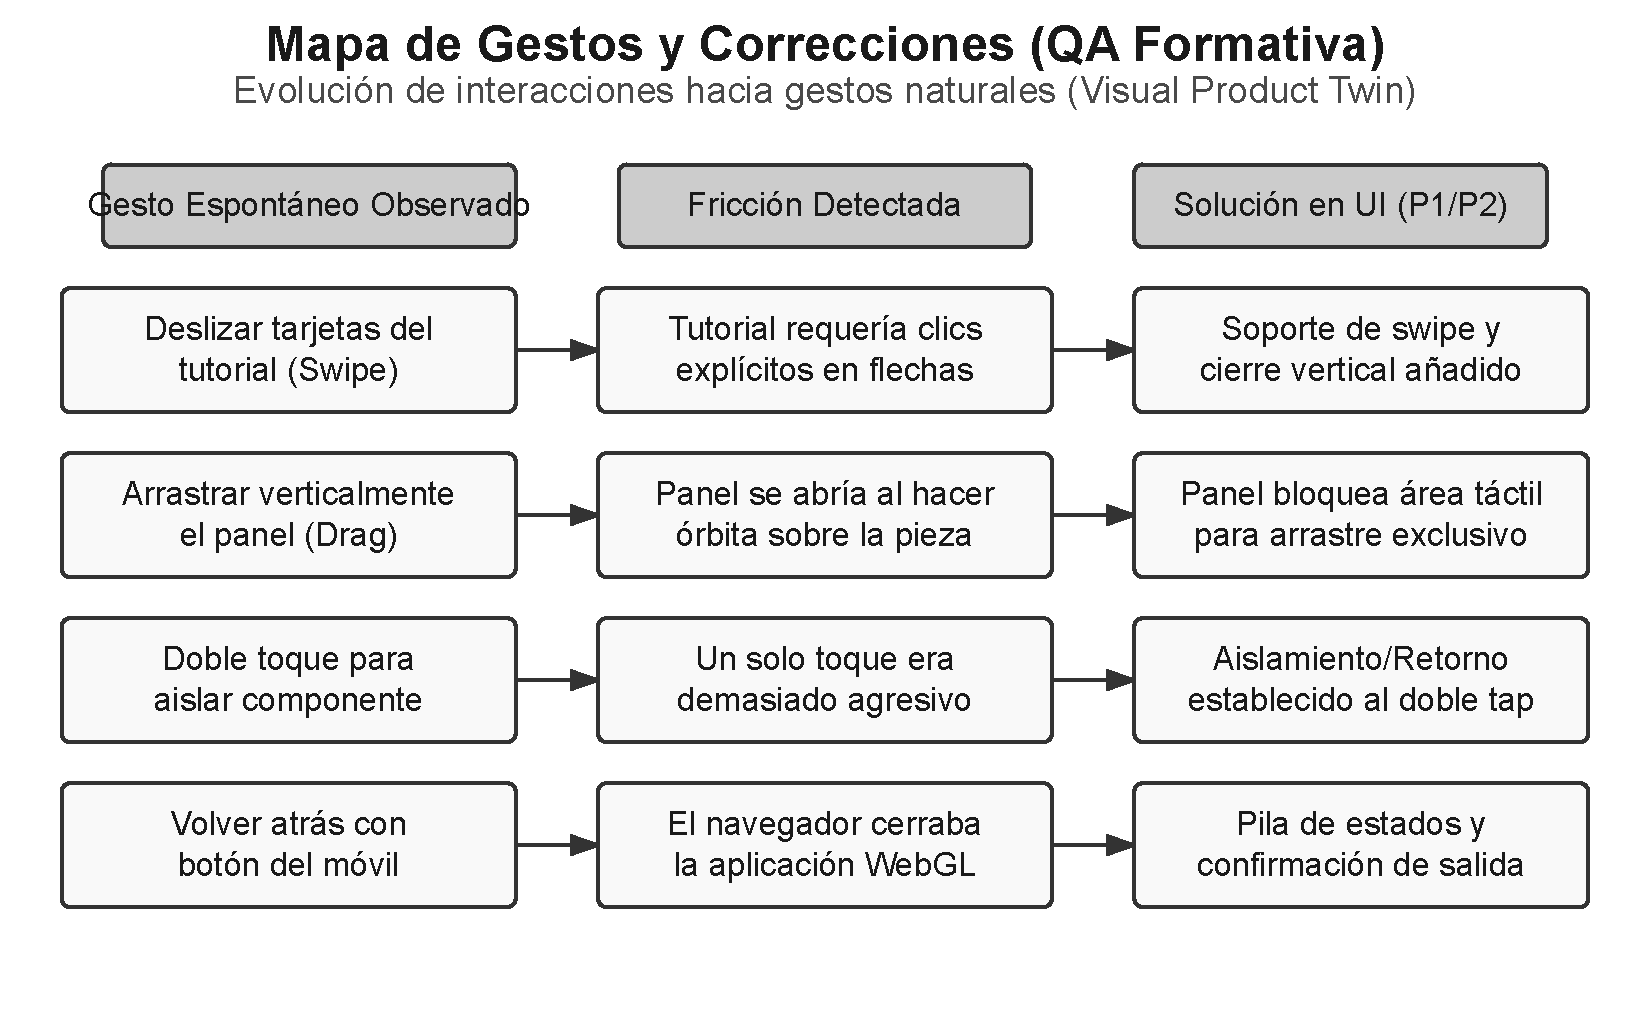
\includegraphics[width=0.88\textwidth,height=0.58\textheight,keepaspectratio]{figures/chapter5/fig_5_mapa_gestos_fixes.pdf}
    \par\vspace{0.5\baselineskip}
    \apanote{Mapeo visual que conecta las fricciones de interacción táctil identificadas en la prueba previa de Think-Aloud con sus correspondientes soluciones implementadas en la interfaz de la build. Elaboración propia.}
\end{figure}

\subsection{Resultados de usabilidad}

La evaluación de usabilidad se aplicó a 12 participantes anonimizados entre el 20 de mayo y el 3 de junio de 2026. Diez participantes realizaron la prueba en smartphone y dos participantes la realizaron en PC; en todos los casos se utilizó Google Chrome. Las pruebas móviles se ejecutaron en un Redmi Note 10S con MIUI Global 14.0.11 y Google Chrome 148. Las dos sesiones de escritorio se realizaron en el mismo equipo empleado para las pruebas técnicas: Intel Core i7-5820K, NVIDIA GTX 980 Ti, 48 GB RAM, resolución efectiva del viewport de 1910\(\times\)903, Windows 11 y Google Chrome 141. La evaluación con usuarios se ejecutó sobre la misma build usada para la recolección de datos técnicos; en la copia pública de cierre, dicha build queda trazada por la rama \texttt{master}, la URL publicada y los artefactos versionados en \texttt{docs/Build}, \texttt{Informe\_final/} y \texttt{Telemetria/Mediciones\_WebGL}. En todas las sesiones se utilizó la caché del navegador previamente cargada. La secuencia de exposición se contrabalanceó entre visor 3D primero (AB) y soporte 2D primero (BA). La matriz de desempeño registró cuatro tareas equivalentes por condición: ubicación de componente, interpretación funcional, relación espacial y análisis visual guiado. En total se documentaron 96 registros tarea-condición; todos fueron completados, con una ayuda baja en la condición 3D durante la tarea de interpretación funcional del participante 006 (véase la Tabla \ref{tab:desempeno_tareas_condicion}).

\begin{table}[H]
    \caption{Desempeño observado por tarea y condición}
    \label{tab:desempeno_tareas_condicion}
    \centering
    \scriptsize
    \singlespacing
    \renewcommand{\arraystretch}{1.08}
    \setlength{\tabcolsep}{3pt}
    \begin{tabular}{p{3.1cm}p{2.2cm}p{2.2cm}p{2.4cm}p{4.3cm}}
        \hline
        \textbf{Tarea} & \textbf{Visor 3D} & \textbf{Soporte 2D} & \textbf{Errores / ayudas} & \textbf{Lectura} \\ \hline
        T1. Ubicación de componente & 12/12 completadas & 12/12 completadas & 0 errores; 0 ayudas & Los participantes localizaron el motor y piezas cercanas en ambas condiciones. \\
        T2. Interpretación funcional & 12/12 completadas & 12/12 completadas & 0 errores; 1 ayuda baja en 3D & El \textit{bottom sheet} permitió consultar información de pieza; un caso requirió repetir la instrucción. \\
        T3. Relación espacial & 12/12 completadas & 12/12 completadas & 0 errores; 0 ayudas & La relación motor--montura--tornillería fue resuelta en ambos medios, con mayor claridad cualitativa atribuida al visor 3D. \\
        T4. Análisis visual guiado & 12/12 completadas & 12/12 completadas & 0 errores; 0 ayudas & En 3D se usaron vista explosionada, \textit{X-Ray} y presets visuales; en 2D se interpretó la información estática equivalente. \\ \hline
    \end{tabular}
    \par\vspace{0.5\baselineskip}
    \apanote{La tabla sintetiza los registros estructurados del moderador por tarea y condición. La lectura cualitativa complementaria se presenta en la sección de \textit{Think-Aloud}. Elaboración propia.}
\end{table}

La medición temporal se aplicó a T1, T2 y T3, porque estas tareas tenían inicio y cierre claramente comparables entre visor 3D y soporte 2D. La T4 se mantuvo como tarea exploratoria guiada y, por esa razón, no se cronometró ni se incluye en el análisis temporal. Su lectura se conserva en la observación cualitativa y en el protocolo \textit{Think-Aloud}. Los tiempos se registraron como cronometraje operativo en segundos durante la sesión moderada; por ello se interpretan como evidencia descriptiva de desempeño y no como medición instrumental de alta precisión temporal.

\begin{table}[H]
    \caption{Tiempos registrados por participante en tareas cronometradas}
    \label{tab:tiempos_tareas_cronometradas_participante}
    \centering
    \scriptsize
    \singlespacing
    \setlength{\tabcolsep}{3pt}
    \begin{tabular}{p{1.1cm}p{0.8cm}p{1.7cm}rrrrrr}
        \hline
        \textbf{Código} & \textbf{Sec.} & \textbf{Disp.} & \textbf{T1 3D} & \textbf{T1 2D} & \textbf{T2 3D} & \textbf{T2 2D} & \textbf{T3 3D} & \textbf{T3 2D} \\ \hline
        P001 & AB & Smartphone & 5 & 13 & 3 & 18 & 15 & 23 \\
        P002 & BA & Smartphone & 5 & 13 & 3 & 18 & 11 & 23 \\
        P003 & AB & Smartphone & 5 & 13 & 3 & 18 & 11 & 23 \\
        P004 & BA & PC & 5 & 13 & 3 & 18 & 11 & 23 \\
        P005 & AB & Smartphone & 5 & 13 & 9 & 18 & 11 & 23 \\
        P006 & BA & Smartphone & 5 & 13 & 3 & 18 & 11 & 23 \\
        P007 & AB & Smartphone & 5 & 13 & 3 & 18 & 11 & 23 \\
        P008 & BA & Smartphone & 5 & 13 & 3 & 18 & 11 & 23 \\
        P009 & AB & Smartphone & 14 & 13 & 3 & 18 & 11 & 23 \\
        P010 & BA & Smartphone & 5 & 13 & 3 & 18 & 11 & 23 \\
        P011 & AB & Smartphone & 5 & 13 & 3 & 18 & 11 & 23 \\
        P012 & BA & PC & 5 & 13 & 3 & 18 & 11 & 23 \\ \hline
    \end{tabular}
    \par\vspace{0.5\baselineskip}
    \apanote{Los tiempos se presentan en segundos. Sec. = secuencia de exposición; AB = visor 3D primero y soporte 2D después; BA = soporte 2D primero y visor 3D después. Elaboración propia a partir de los registros del moderador.}
\end{table}

\begin{table}[H]
    \caption{Resumen descriptivo de tiempos en tareas cronometradas}
    \label{tab:resumen_tiempos_tareas_cronometradas}
    \centering
    \small
    \begin{tabular}{p{2.5cm}rrrrp{4.0cm}}
        \hline
        \textbf{Tarea} & \textbf{Media 3D} & \textbf{Media 2D} & \textbf{Dif. 2D--3D} & \textbf{n} & \textbf{Lectura} \\ \hline
        T1 & 5,75 s & 13,00 s & 7,25 s & 12 & Favorable al visor 3D. \\
        T2 & 3,50 s & 18,00 s & 14,50 s & 12 & Favorable al visor 3D. \\
        T3 & 11,33 s & 23,00 s & 11,67 s & 12 & Favorable al visor 3D. \\
        \textbf{Total T1--T3} & \textbf{20,58 s} & \textbf{54,00 s} & \textbf{33,42 s} & \textbf{12} & \textbf{Menor duración acumulada en 3D.} \\ \hline
    \end{tabular}
    \par\vspace{0.5\baselineskip}
    \apanote{La diferencia se calcula como media del soporte 2D menos media del visor 3D. Elaboración propia.}
\end{table}

En las tres tareas cronometradas, la condición 3D presentó menor tiempo medio que el soporte 2D. El tiempo total medio acumulado en T1--T3 fue de 20,58 s para el visor 3D y de 54,00 s para el soporte 2D, con una diferencia media de 33,42 s a favor del visor. Estos resultados se interpretan de forma descriptiva y complementan la lectura de NASA-TLX Raw, donde el visor 3D también presentó menor carga de trabajo percibida.

El SUS se aplicó únicamente al prototipo 3D, de acuerdo con el diseño metodológico. El puntaje promedio fue 91,88, con mediana de 95,00, mínimo de 60,00, máximo de 100,00 y desviación estándar de 11,24. Frente a la referencia histórica de 68 puntos del instrumento, la distribución observada indica una percepción de usabilidad muy favorable, aunque se interpreta de forma descriptiva por el tamaño y carácter no probabilístico de la muestra (véanse la Tabla \ref{tab:validacion_sus_nasa_participantes}, la Tabla \ref{tab:validacion_resumen_sus_nasa} y la Figura \ref{fig:distribucion_sus}).

\begin{table}[H]
    \caption{Resultados SUS y NASA-TLX Raw por participante}
    \label{tab:validacion_sus_nasa_participantes}
    \centering
    \scriptsize
    \begin{tabular}{p{1.2cm}p{0.9cm}p{1.6cm}p{0.9cm}p{1.3cm}p{1.3cm}p{1.3cm}p{3.4cm}}
        \hline
        \textbf{Código} & \textbf{Sec.} & \textbf{Dispositivo} & \textbf{SUS} & \textbf{NASA 3D} & \textbf{NASA 2D} & \textbf{Dif.} & \textbf{Lectura} \\ \hline
        001 & AB & Smartphone & 90,00 & 7,00 & 17,50 & 10,50 & Usabilidad alta y menor carga en visor 3D. \\
        002 & BA & Smartphone & 95,00 & 5,17 & 17,50 & 12,33 & Usabilidad alta y baja carga 3D. \\
        003 & AB & Smartphone & 97,50 & 8,67 & 22,83 & 14,16 & Diferencia favorable al visor. \\
        004 & BA & PC & 90,00 & 11,17 & 22,50 & 11,33 & Flujo claro también en escritorio. \\
        005 & AB & Smartphone & 90,00 & 7,50 & 24,17 & 16,67 & Carga 2D más alta en comparación. \\
        006 & BA & Smartphone & 60,00 & 25,00 & 36,67 & 11,67 & Caso con mayor fricción, pero menor carga 3D. \\
        007 & AB & Smartphone & 100,00 & 5,83 & 15,00 & 9,17 & Experiencia muy favorable. \\
        008 & BA & Smartphone & 100,00 & 10,83 & 16,67 & 5,84 & Diferencia favorable moderada. \\
        009 & AB & Smartphone & 100,00 & 9,17 & 15,00 & 5,83 & Usabilidad máxima registrada. \\
        010 & BA & Smartphone & 95,00 & 3,50 & 15,00 & 11,50 & Menor carga 3D del grupo. \\
        011 & AB & Smartphone & 85,00 & 5,17 & 16,67 & 11,50 & Resultado favorable con fricciones menores. \\
        012 & BA & PC & 100,00 & 5,33 & 19,17 & 13,84 & Uso fluido en PC. \\ \hline
    \end{tabular}
    \par\vspace{0.5\baselineskip}
    \apanote{Sec. = secuencia de exposición; AB = visor 3D primero y soporte 2D después; BA = soporte 2D primero y visor 3D después. La diferencia se calcula como NASA-TLX Raw 2D menos NASA-TLX Raw 3D. Elaboración propia a partir de los instrumentos de validación aplicados.}
\end{table}

\begin{table}[H]
    \caption{Resumen descriptivo de usabilidad y carga de trabajo percibida}
    \label{tab:validacion_resumen_sus_nasa}
    \centering
    \small
    \begin{tabular}{p{5.0cm}rrrrrr}
        \hline
        \textbf{Medida} & \textbf{n} & \textbf{Media} & \textbf{Mediana} & \textbf{Mín.} & \textbf{Máx.} & \textbf{DE} \\ \hline
        SUS & 12 & 91,88 & 95,00 & 60,00 & 100,00 & 11,24 \\
        NASA-TLX Raw visor 3D & 12 & 8,69 & 7,25 & 3,50 & 25,00 & 5,66 \\
        NASA-TLX Raw soporte 2D & 12 & 19,89 & 17,50 & 15,00 & 36,67 & 6,18 \\
        Diferencia 2D--3D pareada & 12 & 11,19 & 11,50 & 5,83 & 16,67 & 3,16 \\ \hline
    \end{tabular}
    \par\vspace{0.5\baselineskip}
    \apanote{DE = desviación estándar. Los resultados se interpretan de forma descriptiva y exploratoria por el tamaño de muestra y el muestreo no probabilístico. Elaboración propia.}
\end{table}

\begin{figure}[H]
    \caption{Distribución del puntaje SUS en la muestra evaluada.}
    \label{fig:distribucion_sus}
    \centering
    \includegraphics[width=\textwidth,height=0.54\textheight,keepaspectratio]{figures/chapter5/fig_5_sus_distribucion.pdf}
    \par\vspace{0.5\baselineskip}
    \apanote{La línea de referencia marca 68 puntos, valor usado como promedio histórico contextual del instrumento. La lectura del proyecto es descriptiva y no inferencial. Elaboración propia.}
\end{figure}

\subsection{Resultados de carga de trabajo percibida}

La lectura de NASA-TLX Raw confirma una menor carga de trabajo percibida en el visor 3D frente al soporte 2D de referencia. El promedio del visor fue 8,69, mientras que el soporte 2D obtuvo 19,89. La diferencia pareada media fue de 11,19 puntos a favor del visor 3D, y en los 12 casos el valor NASA-TLX Raw fue menor en la condición interactiva. Esta diferencia no se interpreta como prueba inferencial, sino como tendencia descriptiva consistente dentro de la muestra evaluada.

Por dimensiones, el visor 3D presentó menores promedios en demanda mental, demanda física, rendimiento invertido, esfuerzo y frustración; la demanda temporal fue equivalente entre condiciones. Las diferencias más visibles aparecieron en frustración, rendimiento percibido y demanda mental, lo que sugiere que la navegación 3D, la selección contextual y las vistas analíticas redujeron parte del esfuerzo de ubicación espacial requerido por el soporte 2D (véanse la Tabla \ref{tab:nasa_tlx_dimensiones_condicion} y la Figura \ref{fig:nasatlx_dimensiones}).

\begin{table}[H]
    \caption{Promedios NASA-TLX Raw por dimensión y condición}
    \label{tab:nasa_tlx_dimensiones_condicion}
    \centering
    \small
    \begin{tabular}{p{4.6cm}rrr}
        \hline
        \textbf{Dimensión} & \textbf{Visor 3D} & \textbf{Soporte 2D} & \textbf{Diferencia} \\ \hline
        Demanda mental & 10,58 & 25,00 & 14,42 \\
        Demanda física & 4,08 & 5,58 & 1,50 \\
        Demanda temporal & 10,00 & 10,00 & 0,00 \\
        Rendimiento invertido & 3,33 & 23,75 & 20,42 \\
        Esfuerzo & 19,58 & 27,50 & 7,92 \\
        Frustración & 4,58 & 27,50 & 22,92 \\ \hline
    \end{tabular}
    \par\vspace{0.5\baselineskip}
    \apanote{La dimensión de rendimiento se registró con escala invertida: 0 = perfecto y 100 = fallido. Por ello, valores menores indican mejor percepción de desempeño. Elaboración propia.}
\end{table}

\begin{figure}[H]
    \caption{Comparativa NASA-TLX Raw por dimensiones.}
    \label{fig:nasatlx_dimensiones}
    \centering
    \includegraphics[width=\textwidth,height=0.54\textheight,keepaspectratio]{figures/chapter5/fig_5_nasatlx_dimensiones.pdf}
    \par\vspace{0.5\baselineskip}
    \apanote{La figura compara los promedios por dimensión para el visor 3D y el soporte 2D de referencia. Valores menores representan menor carga de trabajo percibida. Elaboración propia.}
\end{figure}

La convergencia entre menor NASA-TLX Raw, menor tiempo medio en T1--T3 y verbalizaciones orientadas a comprensión espacial sugiere que el valor del visor no se concentró en una sola métrica. La evidencia apunta a una experiencia en la que la interacción 3D ayudó a localizar, relacionar y consultar componentes con menor esfuerzo percibido, aunque la lectura se mantiene descriptiva por el tamaño y tipo de muestra.

\subsection{Resultados cualitativos}

El protocolo \textit{Think-Aloud} permitió triangular los puntajes cuantitativos con verbalizaciones, observación de tareas y comentarios posteriores. La categoría más recurrente fue comprensión espacial, presente en 11 de los 12 participantes, seguida de navegación y control en 10 participantes. Esto es coherente con la naturaleza del prototipo: los usuarios valoraron la posibilidad de entender relaciones entre motor, montura, tornillería y modos de visualización, pero también registraron fricciones propias de la interacción táctil y de la selección de piezas pequeñas.

Los temas de mejora más repetidos fueron inconsistencias visuales o estados incorrectos en iconos procedurales (6 participantes), problemas ocasionales de navegación móvil con órbita o \textit{pan} (5 participantes) y dificultad para seleccionar piezas pequeñas o parcialmente ocultas (2 participantes). En contraste, los momentos de claridad se asociaron con el \textit{bottom sheet}, el aislamiento, la vista explosionada, \textit{X-Ray}, \textit{Blueprint} y la visualización térmica. La Tabla \ref{tab:thinkaloud_sintesis} resume la codificación cualitativa y la Figura \ref{fig:thinkaloud_codificacion} la representa de forma visual.

\begin{table}[H]
    \caption{Síntesis de hallazgos \textit{Think-Aloud}}
    \label{tab:thinkaloud_sintesis}
    \centering
    \scriptsize
    \begin{tabular}{p{3.5cm}p{1.9cm}p{5.8cm}p{2.4cm}}
        \hline
        \textbf{Categoría analítica} & \textbf{Frecuencia} & \textbf{Evidencia representativa} & \textbf{Lectura} \\ \hline
        Comprensión espacial & 11/12 & Participantes usaron el visor para relacionar motor, montura, tornillería y disposición del conjunto. & Fortaleza principal del prototipo. \\
        Navegación y control & 10/12 & En móvil se repitieron fricciones con órbita, \textit{pan} y sensibilidad táctil. & Punto de mejora UX móvil. \\
        Percepción de claridad & 8/12 & Vista explosionada, vista térmica, \textit{X-Ray}, \textit{Blueprint} y aislamiento facilitaron la lectura técnica. & Apoya la reducción de carga percibida. \\
        Interpretación de interfaz & 7/12 & La lectura de iconos, menús y estados visuales concentró dudas y comentarios de mejora. & Requiere pulido visual continuo. \\
        Estrategias de recuperación & 3/12 & Algunos usuarios cambiaron de ángulo, repitieron gestos o usaron capas de navegación para resolver dudas. & Indica aprendizaje durante la sesión. \\
        Errores, bloqueos o dudas & 2/12 & La selección de piezas pequeñas o parcialmente ocultas generó fricción en casos específicos. & Riesgo localizado en elementos pequeños. \\ \hline
    \end{tabular}
    \par\vspace{0.5\baselineskip}
    \apanote{La frecuencia indica cantidad de participantes en los que apareció la categoría al menos una vez. Las verbalizaciones se sintetizan de forma anonimizada para preservar solo la información necesaria para el análisis. Elaboración propia.}
\end{table}

\begin{figure}[H]
    \caption{Mapa de codificación cualitativa del protocolo \textit{Think-Aloud}.}
    \label{fig:thinkaloud_codificacion}
    \centering
    \includegraphics[width=\textwidth,height=0.54\textheight,keepaspectratio]{figures/chapter5/fig_5_thinkaloud_codificacion.pdf}
    \par\vspace{0.5\baselineskip}
    \apanote{El mapa sintetiza frecuencia por categoría y lectura interpretativa de las verbalizaciones y observaciones registradas durante la prueba. Elaboración propia.}
\end{figure}

\subsection{Resultados del pipeline de activos}

La comparación de rutas de importación y saneamiento geométrico muestra que el problema principal no era solo reducir triángulos, sino transformar una malla CAD difícil de editar en un activo estable, legible y viable para WebGL. La Tabla \ref{tab:reduccion_geometrica_modelo_total} resume el conteo total de triángulos observado por ruta técnica. La Figura \ref{fig:resultados_geometria_malla_optimizada} complementa esta lectura con evidencia visual de la malla optimizada y su wireframe; la Figura \ref{fig:renderes_caso_holybro_x500} muestra el resultado visual del modelo final con mapas de normales y oclusión ambiental.

\begin{table}[H]
    \caption{Conteo total de triángulos por método de importación y optimización}
    \label{tab:reduccion_geometrica_modelo_total}
    \centering
    \small
    \begin{tabular}{>{\raggedright\arraybackslash}p{3.7cm}>{\raggedright\arraybackslash}p{2.6cm}>{\raggedright\arraybackslash}p{7.8cm}}
        \hline
        \textbf{Método} & \textbf{Triángulos totales} & \textbf{Detalle técnico observado} \\ \hline
        Importación directa & 6\,717\,499 tris & Malla caótica, conexiones en T, vértices repetidos, vértices no soldados y caras repetidas. \\
        MoI3D & 6\,864\,586 tris & Malla más limpia en lectura general, pero con n-gons, conexiones en T, vértices no soldados, vértices repetidos y caras repetidas. \\
        STEPper & 6\,525\,748 tris & Menor cantidad de vértices repetidos y caras repetidas frente a las rutas anteriores, pero con conexiones en T y malla desordenada en triángulos. \\
        Modelo base optimizado & 95\,617 tris & Conteo correspondiente al activo base optimizado y a sus masters principales. No incluye proxies, instancias runtime, assets de apoyo ni renderers adicionales de la escena instrumentada. \\ \hline
    \end{tabular}
    \par\vspace{0.5\baselineskip}
    \apanote{La cifra de 95\,617 triángulos corresponde al modelo base optimizado exportado para la build. No equivale al conteo de escena runtime reportado por el profiler, que puede ser mayor al incorporar instancias, proxies, assets de apoyo, renderers activos y otros recursos necesarios para la interacción. Elaboración propia.}
\end{table}

\begin{figure}[H]
    \caption{Malla optimizada final y lectura de wireframe.}
    \label{fig:resultados_geometria_malla_optimizada}
    \centering
    \includegraphics[width=\textwidth,height=0.52\textheight,keepaspectratio]{figures/screenshots_contextual/fig_cad_bake_low_pair.png}
    \par\vspace{0.5\baselineskip}
    \apanote{La comparación muestra el modelo optimizado y su equivalente en wireframe. Esta evidencia se ubica junto al conteo del activo base optimizado de 95\,617 triángulos para relacionar reducción poligonal, limpieza topológica y legibilidad visual del activo. Elaboración propia.}
\end{figure}

\begin{figure}[H]
    \caption{Renders del dron optimizado con mapas de normales y oclusión ambiental.}
    \label{fig:renderes_caso_holybro_x500}
    \centering
    \includegraphics[width=\textwidth,height=0.72\textheight,keepaspectratio]{figures/screenshots_contextual/fig_render_optimized_drone_stack.png}
    \par\vspace{0.5\baselineskip}
    \apanote{Los renders corresponden al modelo low poly optimizado y permiten verificar que la reducción geométrica conserva una lectura formal adecuada mediante apoyo de mapas de normales y AO. Elaboración propia.}
\end{figure}

\subsection{Nota de cierre}

Los resultados muestran que el prototipo alcanzó un cierre funcional verificable, una reducción geométrica sustancial, rendimiento defendible para el alcance del MVP y una recepción favorable en la evaluación con usuarios. En términos cuantitativos, el SUS promedio fue alto, la carga NASA-TLX Raw fue menor para el visor 3D que para el soporte 2D en los 12 casos registrados y las cuatro tareas equivalentes se completaron en ambas condiciones. En términos cualitativos, los participantes asociaron el mayor valor del sistema con la comprensión espacial del ensamblaje, aunque persisten oportunidades de mejora en navegación móvil, lectura de iconos y selección de elementos pequeños.

\subsection{Discusión}

Los resultados muestran que el prototipo 3D no produjo una ventaja binaria de completitud frente al soporte 2D, porque las cuatro tareas se completaron en ambas condiciones y la matriz de desempeño presentó un efecto techo. Sin embargo, la comparación no quedó vacía: el visor 3D redujo de forma consistente la carga de trabajo percibida y, en las tres tareas cronometradas, presentó menores tiempos medios que la referencia 2D. La evidencia más fuerte del estudio no es una mayor tasa de éxito, sino una interacción espacial menos demandante y más eficiente en términos descriptivos dentro de la muestra evaluada.

Desde la Teoría de la Carga Cognitiva, este patrón puede leerse como una reducción de carga extrínseca más que como un aumento de capacidad intrínseca de resolución: el visor 3D no simplifica el sistema técnico en sí, pero sí externaliza relaciones espaciales que en el soporte 2D exigen reconstrucción mental adicional (Sweller et al., 2019; Hegarty \& Waller, 2004). En esa medida, el hallazgo principal del estudio no es una superioridad absoluta en completitud, sino un apoyo cognitivo más eficiente para tareas de inspección espacial.

Esta lectura es coherente con los resultados de NASA-TLX Raw. El visor 3D obtuvo un promedio de 8,69 frente a 19,89 del soporte 2D y fue menor en los 12 casos observados. Por dimensiones, las mayores diferencias aparecieron en demanda mental, rendimiento invertido y frustración, mientras que la demanda temporal fue equivalente entre condiciones. En conjunto, esto sugiere que la representación interactiva, la selección directa de piezas, el \textit{bottom sheet}, el aislamiento, \texttt{Explode}, \texttt{Cut} y los modos visuales redujeron parte del esfuerzo de reconstrucción espacial que el soporte 2D exige al usuario.

Los tiempos descriptivos refuerzan esa interpretación. En T1, T2 y T3, el visor 3D registró medias de 5,75 s, 3,50 s y 11,33 s, frente a 13,00 s, 18,00 s y 23,00 s del soporte 2D. El tiempo total medio acumulado fue de 20,58 s en 3D y de 54,00 s en 2D. Estos datos deben leerse con cautela, porque la muestra fue no probabilística, el diseño fue formativo y no se aplicó estadística inferencial; aun así, complementan de modo consistente la lectura de menor carga percibida en la condición interactiva.

Desde el punto de vista técnico, la build mostró viabilidad clara en escritorio y comportamiento funcional en los dispositivos móviles evaluados, aunque no convirtió la compatibilidad móvil en una garantía universal. La evidencia por dispositivo muestra escritorio estable, comportamiento cercano a la meta en gama media-alta y restricciones en el límite inferior móvil. Del mismo modo, la reducción a 95\,617 triángulos debe interpretarse como métrica del modelo base optimizado y no como conteo total de escena en runtime, que puede ser mayor por la presencia de instancias, proxies, assets de apoyo y renderers activos.

Estas observaciones delimitan con precisión el alcance académico del artefacto. TwinSight X500 se sostiene como \textit{visual product twin} o modelo visual-semántico de producto: organiza piezas, categorías, vistas analíticas y soporte contextual útil para inspección técnica, pero no integra telemetría en vivo, sincronización con activo físico, \textit{twin manifest} formal ni simulación física calibrada. En consecuencia, el aporte principal de esta tesis no es cerrar un gemelo digital operacional, sino demostrar una vía técnicamente viable y metodológicamente defendible para traducir hardware complejo a una experiencia WebGL usable, interpretable y preparada para madurez futura.

\newpage
